\documentclass[
    style=paintings,
    paper=screen,
    blackslide,
    nopagebreaks,
    fleqn
]{powerdot}

\usepackage[brazil]{babel}
\usepackage[utf8]{inputenc}
\usepackage {graphicx}
\usepackage {grffile}


\pdsetup{
lf=Ep1,
rf=Laboratório de Visão Computacional,
palette=GoldenGate,
theslide=slide~\arabic{slide},
list={itemsep=6pt},
%randomdots,
%dprop={dotstyle=ocircle,linewidth=.25pt},
%dmindots=10,dmaxdots=30,
%dbright=10,
}



\title{Busca em Imagens}
\author{Rafael Lopes \and Rodrigo Okada \and William Mizuta}
\date{
Setembro, 2010
\vfill

\includegraphics[height=.1\slidewidth ]{img/logo_usp_b.ps}

\includegraphics[height=.1\slidewidth ]{img/logo_ime_b.ps}
}
\begin{document}
\maketitle

%\begin{slide}{Linhas gerais}
%\tableofcontents{}
%\setcounter{secnumdepth}{-1}
%\end{slide}

\section[slide=false]{Introdução}
\begin{slide}{Introdução}
\begin{itemize}[type=1]
\item <1-> Busca de imagens por similaridade
\item <2-> Funcionalidades do OpenCV
\end{itemize}
\end{slide}


\section[slide=false]{Métodos}
\begin{slide}{Métodos}
\begin{itemize}[type=1]
\item <1-> Foram utilizados quatro diferentes métodos:
\begin{itemize}[type=1]
\item <2-> Histograma global
\item <3-> Speeded Up Robust Features (SURF)
\item <4-> Momento de janelas
\item <5-> Histograma em janelas
\end{itemize}
\end{itemize}
\end{slide}

\begin{slide}{Histograma global}
\begin{itemize}[type=1]
\item <1-> Método de referência
\end{itemize}
\begin{center}
\includegraphics[width=0.80\linewidth]{img/histograma_global}
\end{center}
\end{slide}


\begin{slide}{SURF}
\begin{itemize}[type=1]
\item <1-> Calcula a similaridade tentando fazer o correlacionamento sobre pontos de interesse
\begin{center}
\includegraphics[width=0.80\linewidth]{img/SURF}
\end{center}
\end{itemize}
\end{slide}


\begin{slide}{Momento de janelas}
\begin{itemize}[type=1]
\item <1-> Divide a imagem em NxN janelas e calcula a diferença pelo momento
das janelas de duas imagens
\begin{center}
\includegraphics[width=0.80\linewidth]{img/momento_de_janelas}
\end{center}
\end{itemize}
\end{slide}


\begin{slide}{Histograma em janelas}
\begin{itemize}[type=1]
\item <1-> Calcula a diferença entre janelas de duas imagens
\begin{center}
\includegraphics[width=0.80\linewidth]{img/histograma_em_janelas}
\end{center}
\end{itemize}
\end{slide}


\section[slide=false]{Resultados e análise}
\begin{slide}{Similaridade - Metodologia da análise}
\begin{itemize}[type=1]
\item <1-> Comparação dos métodos com um \it{ground truth}
\item <2-> Adoção de uma medida para calcular a similaridade entre os resultados 
\item <3-> Cálculo da média e do desvio padrão da nota atribuída para cada imagem de entrada 
\end{itemize}
\pause$$T = \frac{\sum\limits_{i=1}^{10}(10-|l_i-p_i|) * (11-p_i)}{\sum\limits_{i=1}^{10}10*i}$$
\end{slide}


\begin{slide}{Similaridade - Resultados}
\begin{center}

\includegraphics[width=0.80\linewidth]{img/tabela1}
\end{center}
\end{slide}


\begin{slide}{Classificador - curva ROC}
\begin{center}
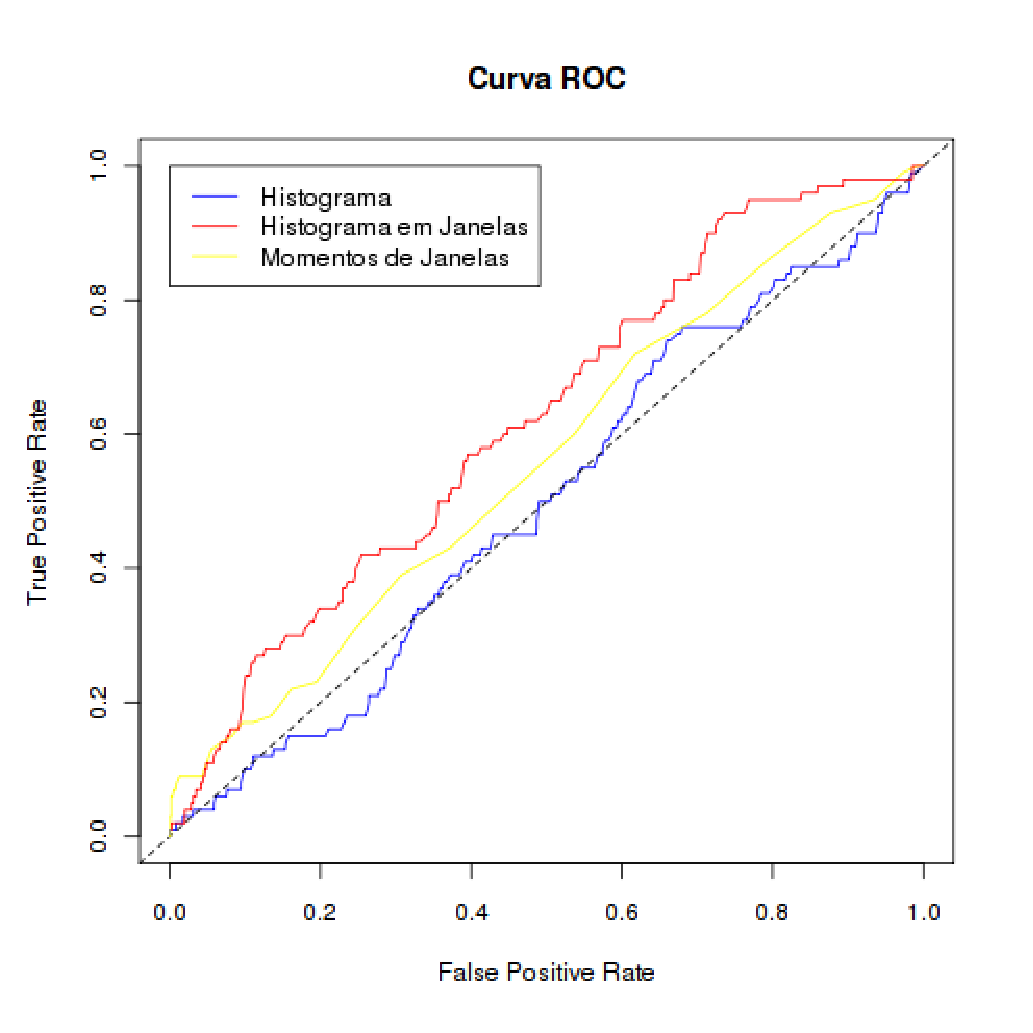
\includegraphics[width=0.65\linewidth]{img/curvaroc}
\end{center}
\end{slide}


\begin{slide}{Classificador - curva Precision X Recall}
\begin{center} 
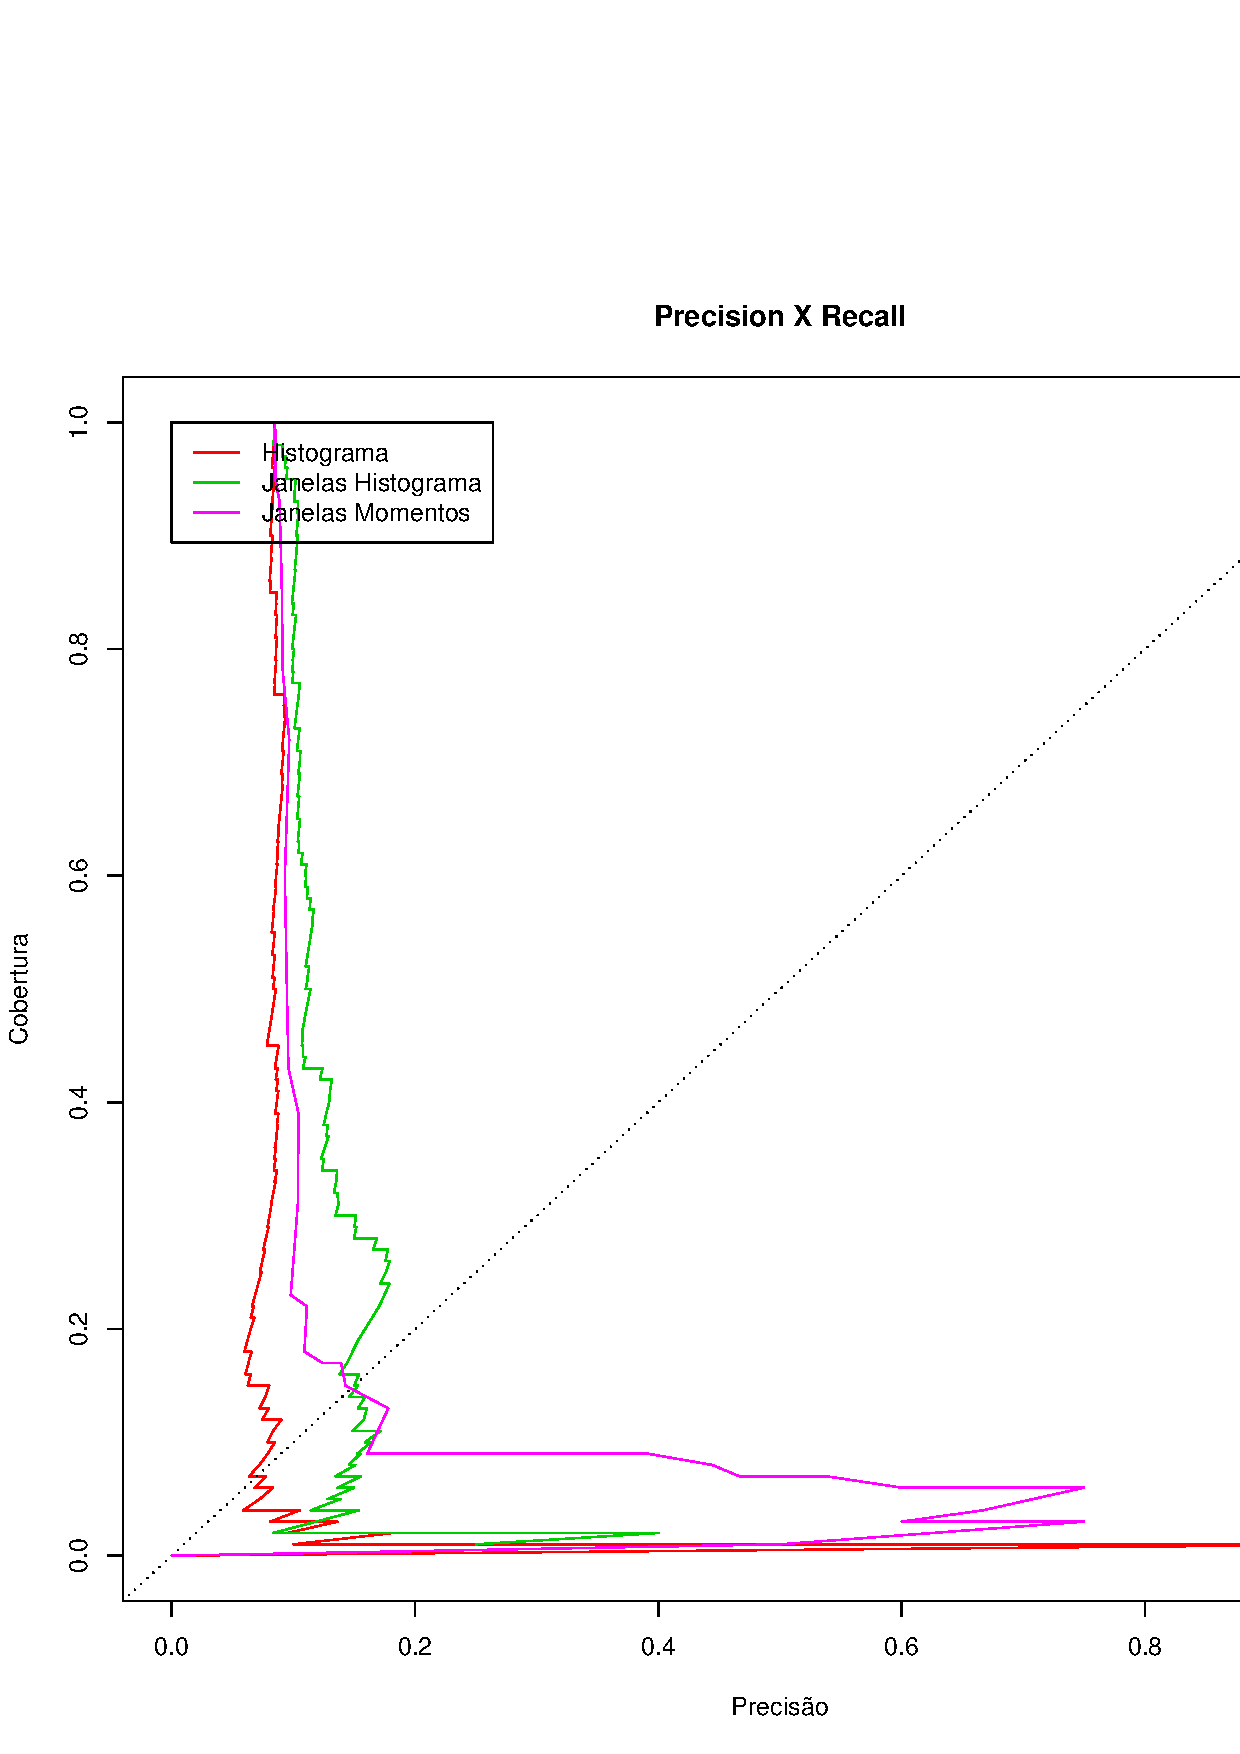
\includegraphics[width=0.65\linewidth]{img/precision_recall}
\end{center}
\end{slide}


\section[slide=false]{Conclusão}
\begin{slide}{Conclusão}
\begin{itemize}[type=1]
\item <1-> O trabalho introduziu os conceitos básicos do OpenCV, exercitando suas funcionalidades básicas
\item <2-> Análise de resultados através de ground truth permite avaliação objetiva de algum método, quantificando sua precisão
\end{itemize}
\end{slide}

%\section[slide=false]{Referências}
%\begin{slide}{Referências}
%\bibliographystyle{plain}
%\bibliography{references}
%\end{slide}


\end{document}
